\annex
\chapter{\hspace{1.2cm}Montagem da panorâmica}

\begin{figure}[ht]
    \caption{Imagens utilizadas para a formação da panorâmica.}     
    \centering
    \vspace{0.3cm}
    \begin{minipage}{.9\textwidth}
      \centering
      \begin{tabular}{cc}
            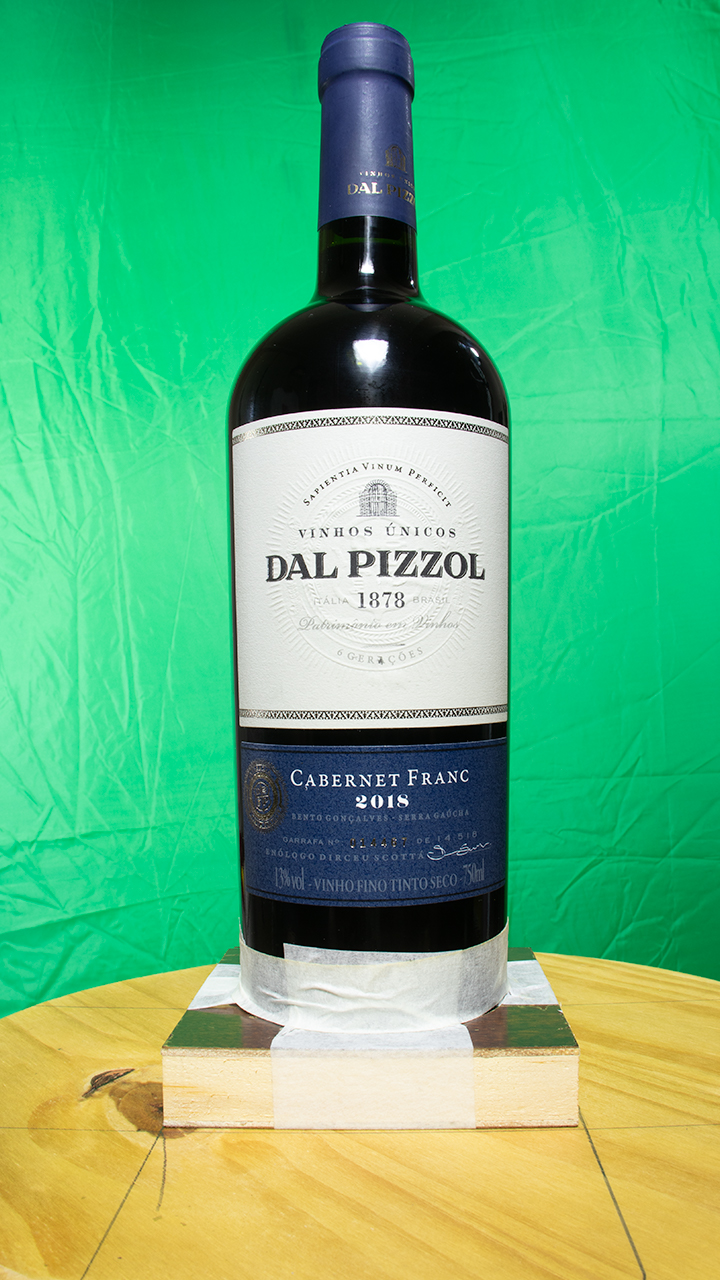
\includegraphics[width=.3\textwidth]{TCC/Imagens/ensaios/0.jpg} 
            &
            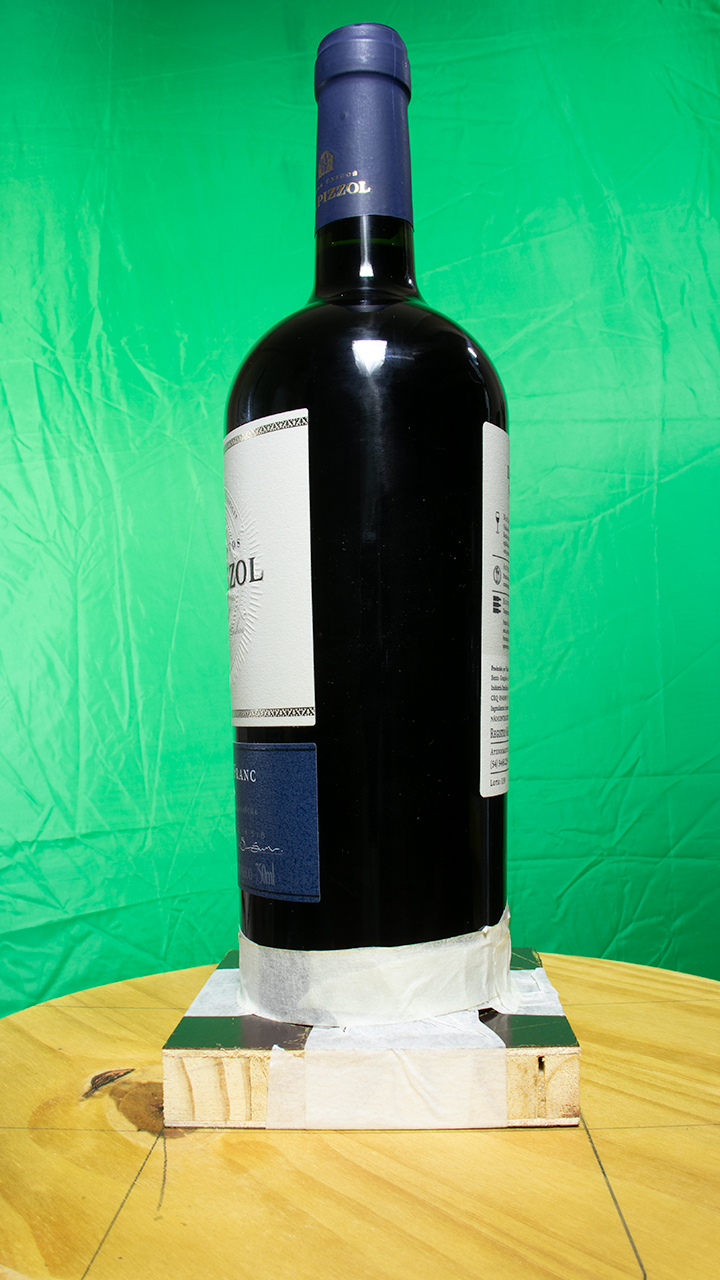
\includegraphics[width=.3\textwidth]{TCC/Imagens/ensaios/90.jpg} \\
            (a) & (b)\\
            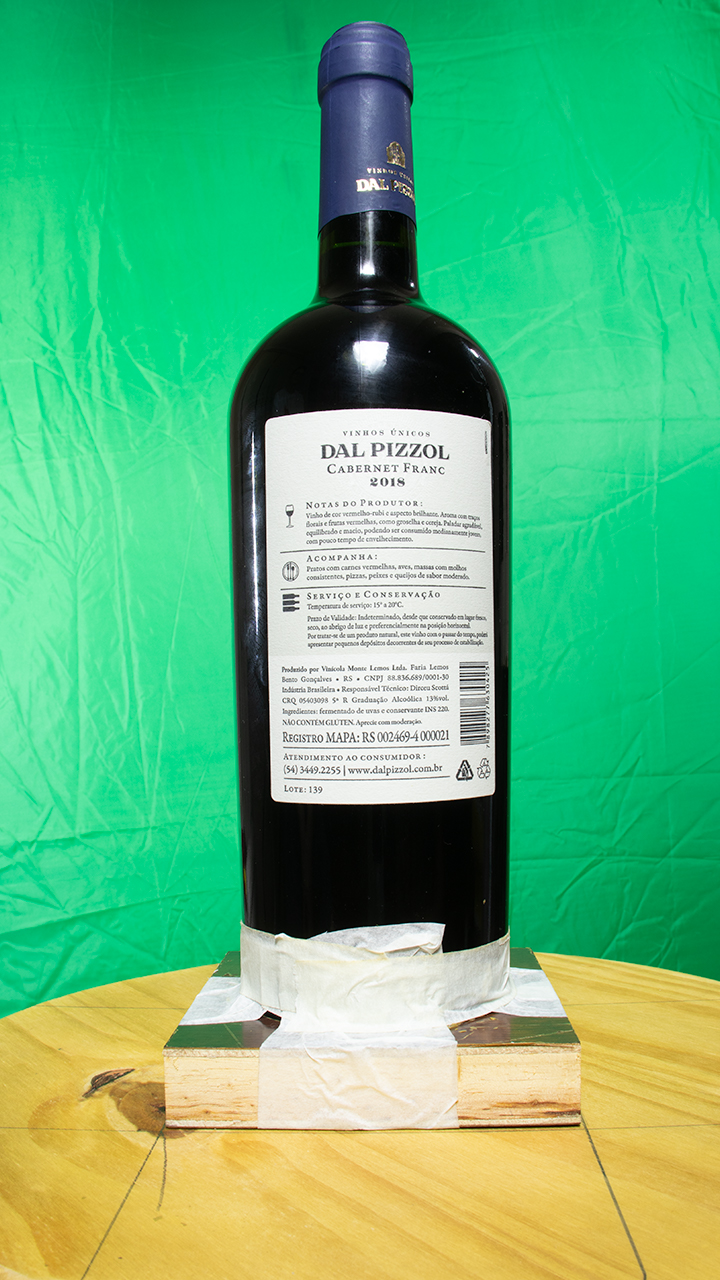
\includegraphics[width=.3\textwidth]{TCC/Imagens/ensaios/180.jpg} 
            &
            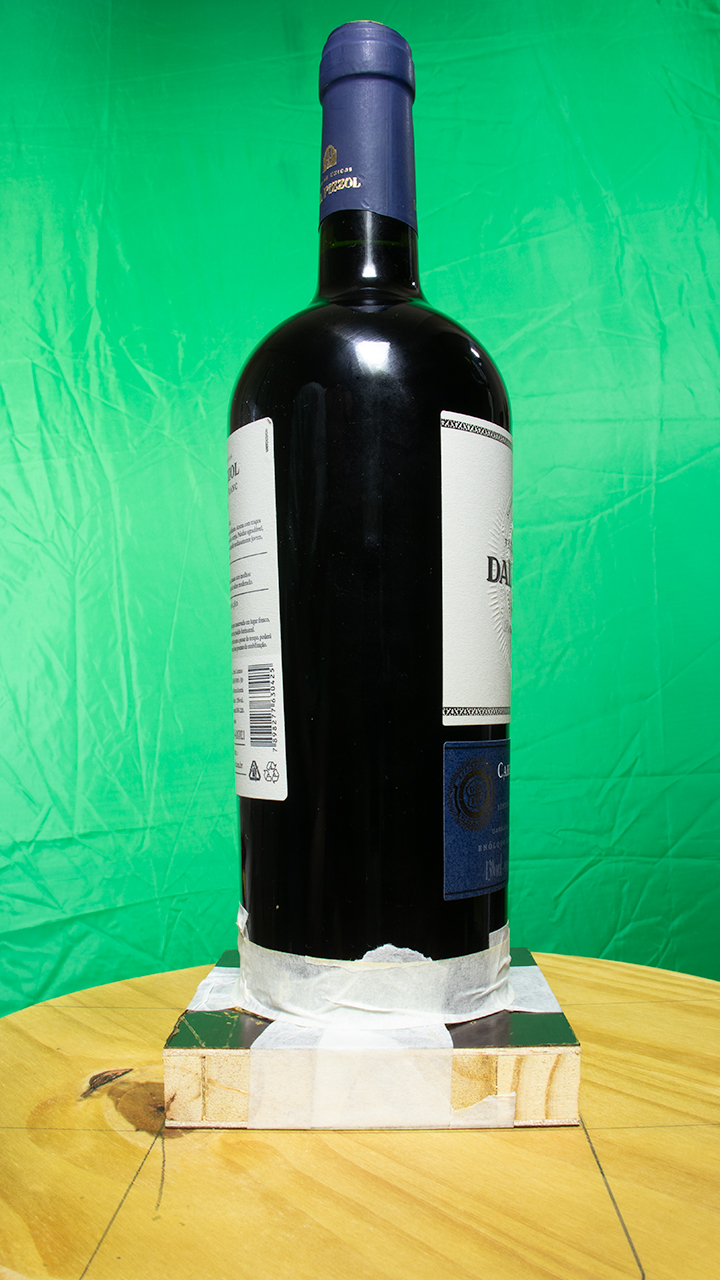
\includegraphics[width=.3\textwidth]{TCC/Imagens/ensaios/270.jpg} \\
            (c) & (d)
            \end{tabular}
            \fonte{O autor, 2020.}
	\end{minipage}
    \label{fig:figs_panoramica}
\end{figure}

% \begin{figure}[ht]
%     \label{fig:figs_panoramica}
%     \centering
%     \caption{Imagens utilizadas para a formação da panorâmica}
%     \vspace{.2cm}
%     \begin{tabular}{cc}
%     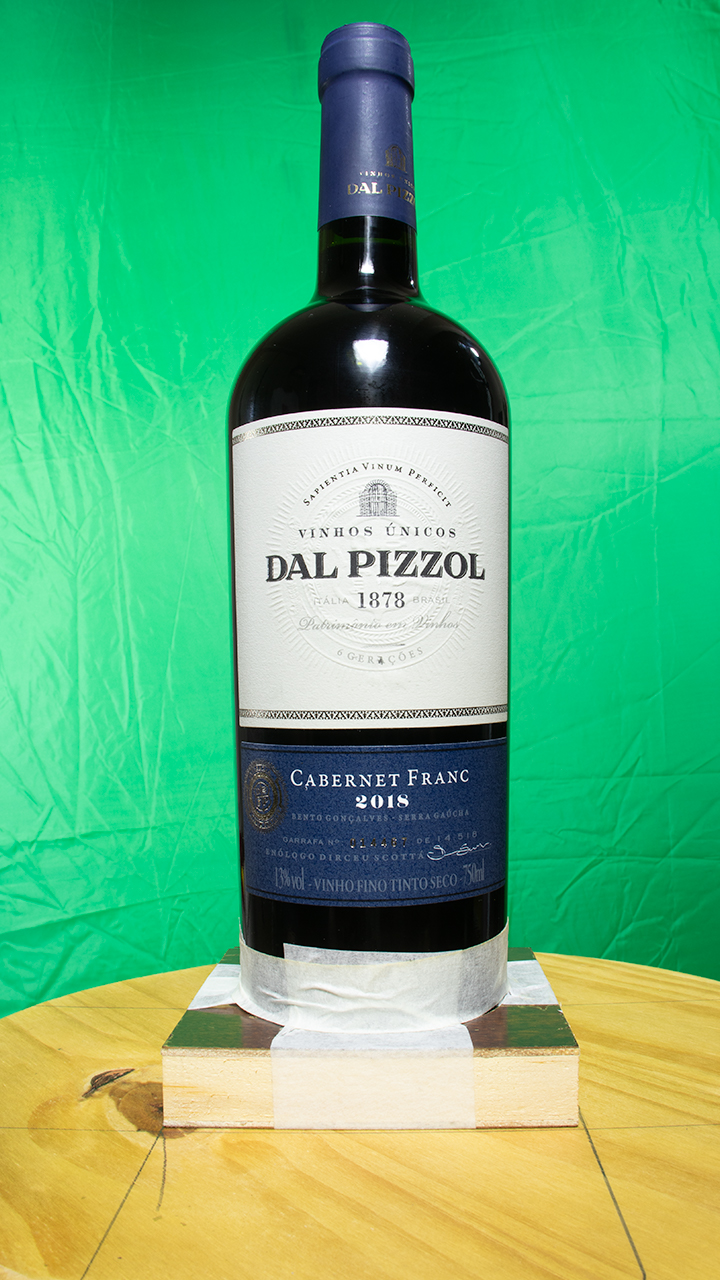
\includegraphics[width=.3\linewidth]{TCC/Imagens/ensaios/0.jpg} 
%     &
%     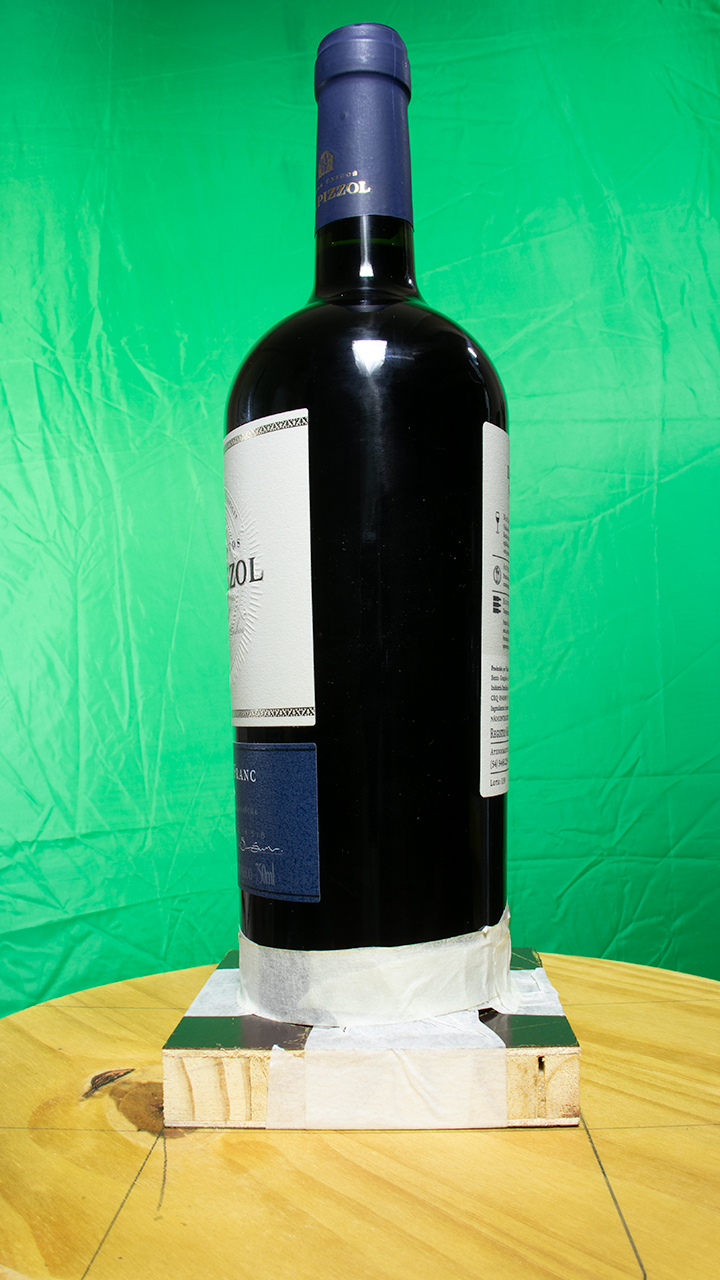
\includegraphics[width=.3\linewidth]{TCC/Imagens/ensaios/90.jpg} \\
%     (a) & (b)\\
%     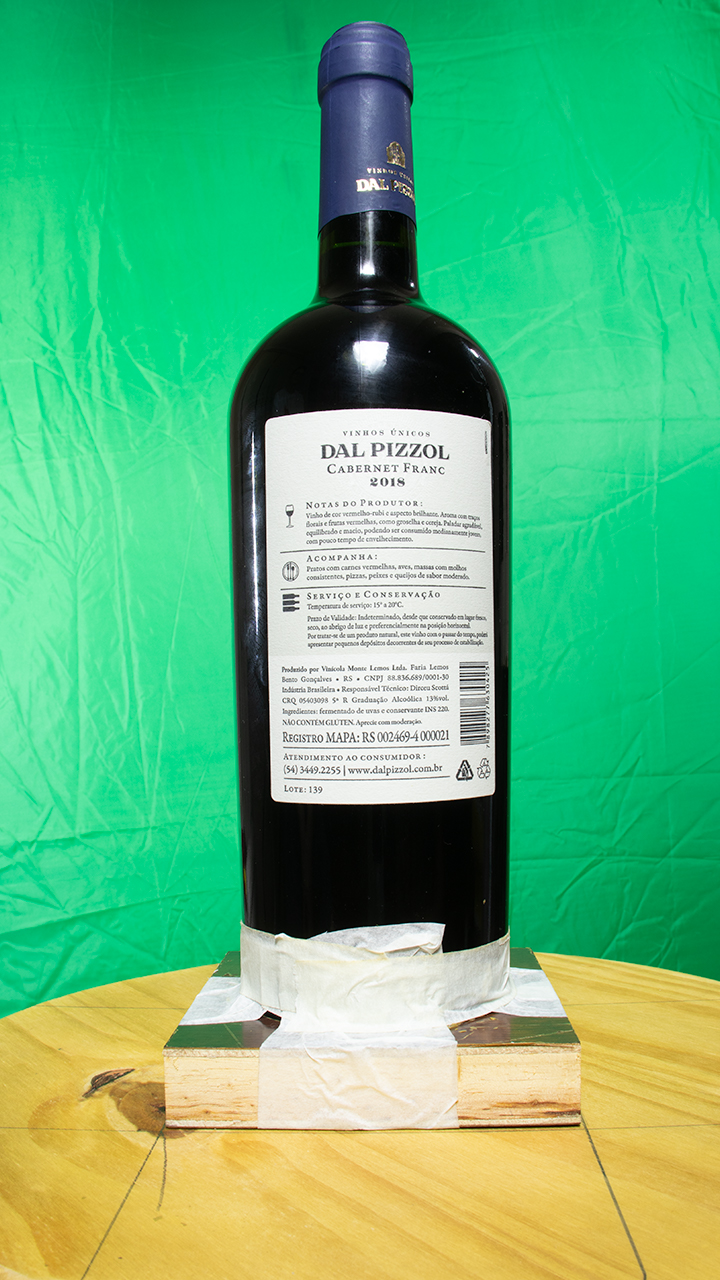
\includegraphics[width=.3\linewidth]{TCC/Imagens/ensaios/180.jpg} 
%     &
%     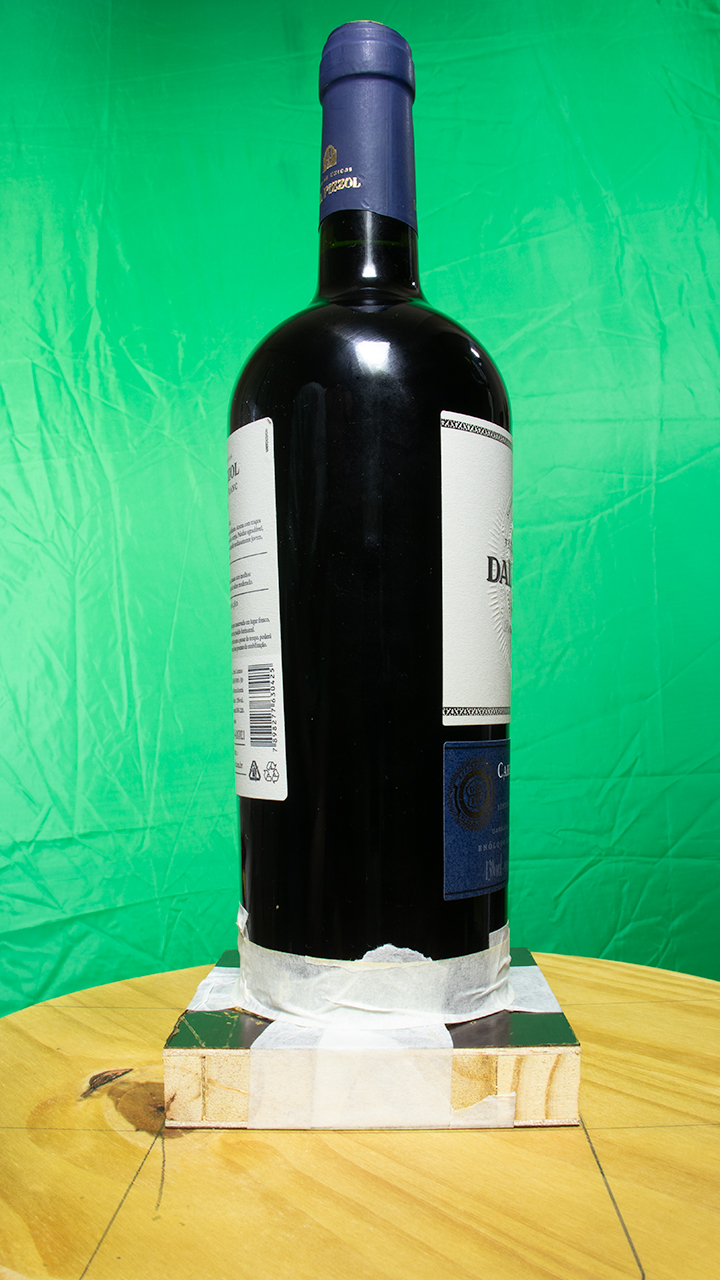
\includegraphics[width=.3\linewidth]{TCC/Imagens/ensaios/270.jpg} \\
%     (c) & (d)
%     \end{tabular}
%     \fonte{O autor, 2020.}    
% \end{figure}


    
